\documentclass[10pt,aspectratio=169]{beamer}


  \usetheme{NYU}      % or try Darmstadt, Madrid, Warsaw, ...
  \usecolortheme{default} % or try albatross, beaver, crane, ...
  \usefonttheme{default}  % or try serif, structurebold, ...
  \setbeamertemplate{navigation symbols}{}
  \setbeamertemplate{caption}[numbered]
\usepackage{appendixnumberbeamer}
\usepackage{mymacro}


\newcommand{\ind}{\perp\!\!\!\!\perp} 
\usepackage{hyperref}
\usepackage{minted}
\usepackage[round]{natbib}

\hypersetup{
    colorlinks=blue,
    linkcolor=blue,
    filecolor=blue,      
    urlcolor=blue,
    citecolor=blue,
}

% If you want to print handouts
%\documentclass[handout]{beamer}

% Changing the fonts: this will make the slides more readable and the math look like regular tex math
%\usefonttheme{arial}

% Titles will appear in Small Cap Serif



% -----------------------------------------
% Center the Frame Title
% -----------------------------------------




% -----------------------------------------
% Number the slides
% -----------------------------------------

\setbeamertemplate{footline}[frame number]

% -----------------------------------------
% Get rid of the irritating navigation bar
% -----------------------------------------

\setbeamertemplate{navigation symbols}{}
% -----------------------------------------
% Begin Document
% -----------------------------------------
\title{\Large\textsc{The Moral Revolution Will Not Be Televised, It Will Be Livestreamed: Censorship and Narrative Control in Mexico}}
\author[Zago] % Esto es lo que sale en el footer
{\textbf{Eduardo Zago}\inst{1}  \vspace{10pt}}

\institute []% Esto es lo que sale en el footer
{  \inst{1}   PhD Student NYU Politics}

\date{\textsc{}}

\titlegraphic{\hfill\includegraphics[height=1.5cm]{nyu_stacked_color}}


\begin{document}
\maketitle
%  I separate each slide with a line:

% -----------------------------------------

%  I start with the screen black, like using the b key in Powerpoint



% -----------------------------------------
%  Restore normal white background

\beamersetaveragebackground{white}


% -----------------------------------------

%  Example of a slide with animated math:
\section{Motivation}


\begin{frame}{Why Governments Hold Interactions with Media?}
\begin{itemize}
  \setlength\itemsep{1em}

    \item Globally, governments increasingly trying to speak \alert{directly} to audiences and to \alert{manage press access} through controlled formats (press pools, livestreams, social media).
    \item President Trump has had more exchanges with the press than 6 predecessors {\footnotesize\color{gray}\citep{Trump100Days}}. 
    \item Also, Andres Manuel Lopez Obrador (AMLO), ex-president of Mexico held 1,423 2-hour press conferences during his tenure.
    \item \textbf{Broadly, I would like to shed some light on what are the incentives (and costs) of both, the government and the media, to have these recurrent interactions?}

    
\end{itemize}
\end{frame}

%%%%%%%%%%%%%%%%%%%%%%%%%%%%%%%%%%%%%%%

\section{Why Mexico?}

\begin{frame}{Mexican Context: Public Money \& Access as Control}

\begin{itemize}
    \setlength\itemsep{0.55em}

    \item \textbf{Mexico is a natural setting to study these interactions:}
    official advertising has long been used to \alert{reward} friendly coverage and \alert{discipline} critics.

\end{itemize}

\vspace{0.2cm}
\begin{quote}
\centering
``Pay for them to beat up on me? Gentlemen, I think not!''

\hfill --- \tiny{President L\'opez Portillo (1982), announcing the withdrawal of advertising from independent media \citep{PrensaVendida-Rod}.}
\end{quote}

\begin{itemize}
    \setlength\itemsep{0.55em}

    \item \textbf{This playbook persisted into modern electoral politics:}
\end{itemize}

\vspace{0.2cm}
\begin{quote}
\centering
``With its enormous advertising budget, Mexican government controls the media.''

\hfill --- \tiny{\citep{Times}.}
\end{quote}

\begin{itemize}
    \setlength\itemsep{0.55em}

    \item \textbf{AMLO reshaped the information environment}
    by sharply cutting official advertising and simultaneously creating the \alert{ma\~nanera}.
\end{itemize}

\end{frame}

\begin{frame}{Why Governments Hold Interactions with Media?}
\begin{itemize}
  \setlength\itemsep{1em}


  \item Following his 2018 victory, President L\'opez Obrador (AMLO) created a direct-to-public communication channel: the \textbf{\textit{Mañanera}}.

  \item The \textit{Mañanera} is a daily agenda-setting press conference where access to the microphone depends heavily on \textbf{visibility and physical proximity} (front rows).

  \item Initially, a ``first-come, first-served'' rule generated \textbf{adverse selection of questioners}: front-row access became concentrated among aligned outlets, limiting critical questioning and undermining perceived credibility.

  \item In April 2022, the administration introduced a \alert{daily seat lottery} for the first three rows to broaden access and restore engagement.
\end{itemize}
\end{frame}

%%%%%%%%%%%%%%%%%%%%%%%%%%%%%%%%%%%%%%%%

\begin{frame}
    \begin{figure}
        \centering
        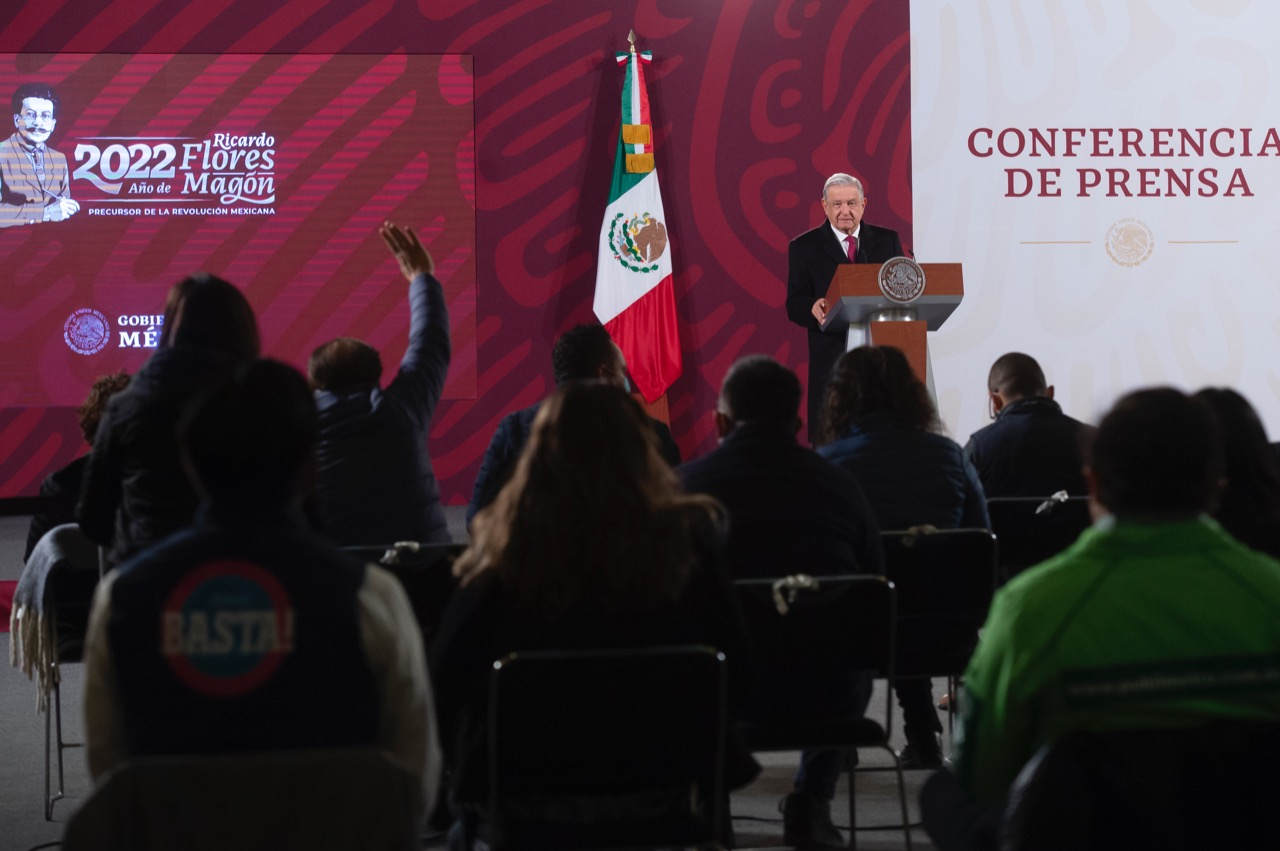
\includegraphics[width=.8\textwidth]{figures/descriptive_stats/mañanera_ex.jpeg}
        \vspace{-0.2cm}
        \caption{\scriptsize Example of a Mañanera}
    \end{figure}
\end{frame}

\section{Why this is important?}

% --- First slide in section: Why this is important? ----------------------------

\begin{frame}{Why the Information Environment Matters}
\begin{itemize}
    \setlength\itemsep{0.65em}

    \item \textbf{Media increases accountability}
    by lowering information frictions, media reporting helps voters \alert{detect} misbehavior and \alert{sanction} incumbents {\footnotesize\color{gray}\citep{Audits-Ferraz-QJE}}.

\item \textbf{Governments spend substantial resources on narrative control} {\footnotesize\color{gray}\citep{ArgCorr-DiTella-AEJAE, MediaCaptures-Zeidl-Econometrica, CensorshipChina-King-Science}}.

    \begin{itemize}
        \item Incumbents understand that
    political survival is linked to what information becomes \alert{salient} and how it is interpreted {\footnotesize\color{gray}\citep{Autocracy-Guriev-JPE}}.
    \item However, persuasion works when \alert{audiences
trust} the information environment {\footnotesize\color{gray}\citep{MediaBias-Gentzkow-JPE}}.
    \end{itemize}
    

    \item \textbf{In autocracies, the playbook is familiar:} \alert{censorship} + \alert{coercion}.
    \begin{itemize}
        \item \textit{Censorship:} China’s online censorship on collective action {\footnotesize\color{gray}\citep{CensorshipCollective-King-APSR}}.
        \item \textit{Coercion:} the murder of Jamal Khashoggi in a Saudi consulate.
    \end{itemize}
\end{itemize}
\end{frame}

\begin{frame}
\frametitle{Censorship in democracies}

\begin{itemize}
 \item \textbf{What about in democracies?}
    Direct repression is costly and often constrained, but government still has techniques to silence critics {\footnotesize\color{gray}\citep{Censor-Pratt-AER}}.
    \vspace{0.2cm}
\item Which instruments are used?

\begin{enumerate}
    \item \textbf{Bribery:} Montesinos in Peru {\footnotesize\color{gray}\citep{Peru-Macmillan-JEP}}.
    \item \textbf{De-legitimization:} South Korea \textit{giraegi} and Trump in US {\footnotesize\color{gray}\citep{KoreaJour-Shin-Journalism, PressCriticism-Carlson-Journalism}}.
    \item \textbf{Restriction of source access:} Kisha clubs in Japan {\footnotesize\color{gray}\citep{Kisha-Freedom}}.
    \item \textbf{Public resource allocation:} Argentina and Hungary governments use \alert{advertising} to \alert{reward} supportive outlets and \alert{discipline} critics {\footnotesize\color{gray}\citep{ArgCorr-DiTella-AEJAE, MediaCaptures-Zeidl-Econometrica}}.
\end{enumerate}

\vspace{0.2cm}
\item \textbf{How effective are they?}
\begin{itemize}
  \item \alert{Not Clear!} We rarely observe clean exogenous variation in exposure to dissent and government responses, causal identification is rare for most of these.
\end{itemize}
\end{itemize}
\end{frame}

\begin{frame}{What this paper adds (Cont.)}
\begin{itemize}\setlength\itemsep{0.85em}

\item \textbf{Why the literature gets stuck:}
  \begin{itemize}\setlength\itemsep{0.25em}
    \item \textbf{Dissent is usually endogenous:} aligned outlets self-select into access and favorable treatment
    {\footnotesize\color{gray}\citep{ArgCorr-DiTella-AEJAE}}.
    \item \textbf{Credible commitment is hard to observe:} we rarely see reforms that plausibly change
    \textit{who can speak} and \textit{how they are rewarded} in a way that can be brought to the data.
    \item \textbf{Credibility is hard to measure:} we rarely observe clean proxies for audience attention in government messaging
    {\footnotesize\color{gray}\citep{PersuasionEmpirical-Dellavigna-AR}}.
  \end{itemize}
  
  \item \textbf{What my setting lets me do:}
  A daily seat lottery provides quasi-random variation in \alert{access to the mic},
  and rich administrative data let me trace its consequences. At the moment, provide reduced form short term causal evidence on:
  \begin{itemize}\setlength\itemsep{0.25em}
    \item \textbf{private advertising} benefits of media companies from interacting with the government (via YouTube metrics, Twitter, Google Trends), and
    \item censorship decisions of the government through the allocation of \textbf{state advertising} (via COMSOC contracts).
  \end{itemize}
\end{itemize}
\end{frame}

\section{Empirical Strategy}

\begin{frame}{How the Seat Lottery Works}
\begin{itemize}
  \setlength\itemsep{0.8em}

  \item After April 2022, access to the \alert{first three rows} started depending on \alert{daily lottery} among accredited attendees.

  \item The lottery is \alert{stratified by media type}: seats are drawn separately within categories (e.g., print, TV, radio, digital), and then assigned to the front rows.

  \item Rotation rule: outlets that asked a question the day before are excluded from the lottery.

  \item My identifying claim is simple: \alert{within day $\times$ media type $\times$ not-asked-yesterday}, who lands in the first rows is as-good-as random.
\end{itemize}
\end{frame}

\begin{frame}{Relevance: lottery shifts who gets the mic and what gets aired}
\small
\begin{itemize}\setlength\itemsep{0.65em}

  \item \textbf{Seat location predicts voice.}
  In a hand-coded sample of 10 randomly selected conferences, the distribution of questions by row is:
  \[
  \text{Row 1: }71\% \quad\text{Row 2: }20\% \quad\text{Row 3: }4.5\% \quad\text{Other: }4.5\%.
  \]

  \item \textbf{Implication: it shifts the on-air ``question market.''}
  If being in the first rows is the main bottleneck, randomizing those seats should:
  \begin{itemize}\setlength\itemsep{0.35em}
    \item \alert{deconcentrate} question access (fewer outlets monopolizing the mic), and
    \item increase the probability that \alert{more critical outlets} are the ones whose questions become salient on air.
  \end{itemize}

  \item \textbf{What this buys me empirically:}
  lottery-induced variation in \emph{who} gets front-row visibility generates quasi-random variation in \emph{who} gets to ask, conditional on attending.

\end{itemize}
\end{frame}

\begin{frame}
  \centering
  
\includegraphics[width=\linewidth]{figures/descriptive_stats/outlet_density2.pdf}

  \vspace{0.4em}
  \scriptsize
  \begin{tabular}{l}
  \end{tabular}

\vspace{0.35em}
\centering
\scriptsize
% If the table is too large, keep it as a separate slide. If it fits, include it here:
% \vspace{0.2em}
% \input{tables/top10_outlets_before_after.tex}
\end{frame}

%%%%%%%%%%%%%%%%%%%%%%%%%%%%%%%%%%%%%%%%%%

\begin{frame}

\begin{table}[!htpb]
    \centering
    \scriptsize
    \caption{Top 10 Outlets that Asked the Most Questions}
    \label{tab:outlets}
    \begin{tabular}{cccc}
\hline \\
Outlet (Before) & Questions (Before) & Outlet (After) & Questions (After) \\
\hline\\
Grupo Healy & 72 &  Grupo Healy & 32 \\
 A Tiempo TV  & 42 &  La Crónica & 31 \\
 Tabasco Hoy & 40 & Frontera & 30 \\
 Campeche Hoy & 39 &  Contralínea & 29 \\
 Quintana Roo Hoy\footnote{\tiny Widely considered 'southern friendly outlets' of the government (\href{https://animalpolitico.com/verificacion-de-hechos/te-explico/amlo-medios-promesas-publicidad-oficial}{Animal Político})} & 37 &  SDP Noticias & 28 \\
Frontera & 35 &  Proceso\footnote{\tiny AMLO of Proceso: '\textit{Conservative journalism, serving corrupt minorities, either directly or indirectly, consciously or unconsciously.}'}  & 28 \\
 diario Basta\footnote{\tiny Diario Basta CEO: 'Thanks to my friend and fellow countryman, President López Obrador, for his support throughout his administration to @diariobasta and @grupocanton. Love is repaid with love.'} & 33 &  Canal 11 & 25 \\
 La Crónica & 32 &  El Financiero\footnote{\tiny AMLO to a Financiero journalist: '\textit{I don't want to get involved in that. Why should I give a story to your newspaper if you're against us?}'} & 22 \\
 Contralínea & 29 &  Noticiero en Redes. & 18 \\
 Imagen del Golfo  & 28 &  Tabasco Hoy & 16 \\
\hline
\end{tabular}
\end{table}
\end{frame}

%%%%%%%%%%%%%%%%%%%%%%%%%%%%%%%%%%%%%%%%%%%%%%%%%%%%%%%%%%%%%

\begin{frame}{Setup}\frametitle{Set up and Model}
\small
\textbf{Data.} For each day $t$ and outlet $i$: (a) attendance indicator; (b) who asked;  (d) outcome; (e) media alignment.

\medskip
\textbf{Variables.} Let $D_{it}=1$ if outlet $i$ asked a question at time $t$; let $\Delta Y_{i,t+h}$ be media viewership at time $t$; $Attend_{it}$ be the number of times each outlet attended the conference in the relevant time period.

\medskip
\textbf{Specification.} With outlet and time fixed effects:
\[
\underbrace{ Y_{i,t}}_{\text{Media viewership}}
\;=\;
\beta\,D_{it}
\;+\;
\lambda\,\textit{Attend}_{it}
\;+\;
X'_{it}\theta
\;+\;
\alpha_i
\;+\;
\tau_t
\;+\;
\varepsilon_{it}
\]

\medskip

\end{frame}

%-----------------------------------------------

\begin{frame}{Estimation}\frametitle{Estimation}
\small


\begin{itemize}\setlength\itemsep{0.65em}
    \item Following \citet{LiuEtAl}, I will estimate the model using a counterfactual estimator.
    \item Use data under the control condition to build models and impute counterfactuals of treated observation.
    \item Avoids negative weights problem (heterogeneous treatment effects)
    \item More efficient than the event-by-event estimators \citep{Borusyak-DIDImp}
    \item Addresses the intermittent treatment case (general panel structure)
\end{itemize}



\medskip

\end{frame}

\begin{frame}{Design 2: Identification}

\small

Following \citet{LiuEtAl}, identification rests on these assumptions:

\begin{itemize}\setlength\itemsep{0.65em}
    \item \emph{Strict exogeneity}: past outcomes do not directly affect current treatment assignment. Condenses (along the functional form one) into:

    $$Y_{is}(0) \ind D_{it} \; | X_{i,1,...,T}, U_{i, 1, ..., T}$$
    \medskip
    \item \alert{Importance of lottery:} 
    \begin{enumerate}\setlength\itemsep{0.65em}
        \item past advertising rewards do not affect selection into asking a question
        \item treatment exogenous to time-varying unobserved confounders. 
        \item the only observed confounder (attendance) correlated with treatment is controlled for
        
    \end{enumerate}
    \medskip
    
    \item Before the lottery, these two would probably be unrealistic assumptions

\end{itemize}

\medskip


\end{frame}

\begin{frame}{Identification}\frametitle{}

\small
\begin{itemize}\setlength\itemsep{0.65em}

    \medskip
    \item \emph{No anticipation and no carry-over effects}: treatment affects contemporaneous outcomes only, not past and future periods. 

    $$D_{t} \ind \{Y_{t-e}, Y_{t+e}\}^{e = 1}_{F}$$
    \item Randomization guarantees no anticipation.
    \item No carry-over effects is testable and plausible for at least private advertising outcomes.
    \item Effects of really viral/salient questions should dissipate at the time period defined (weeks).
    \item Then I just capture the reduced-form \alert{uptick in viewership} from asking a question to the executive.

    
\end{itemize}

\textbf{Interpretation.} $\beta$ is the AITC % average instant effect of changes in treatment
of a \emph{question} on ad spending/revenue, conditional on attendance.

$$AITC = \mathbf{E}[\delta_{it} \, | \, (D_{it} = 0, D_{it} = 1) \; or \; (D_{i,t} = 1, D_{i, t+1})]$$

\end{frame}

\begin{frame}{Identification}\frametitle{Heterogeneity}

\small

\begin{itemize}\setlength\itemsep{0.65em}

    \medskip
    \item At the moment: reduced form (short-term) effects of \alert{asking a question} to the President on private advertising proxies.
    \item I am interested in capturing also the effects of alignment and dissent on both: private advertising revenue and public advertising revenue.
    \item The idea would be to split the dataset into aligned vs. oppositional outlets and estimate the models for each subset. Two additional assumptions are required for interpretability:
    \begin{enumerate}
        \item \textbf{media alignment is constant across the study time}: could provide some pre-loterry evidence of this using questions asked/proportion of critical articles/tweets/etc.
        \item \textbf{oppositional media do not ask aligned questions, and viceversa}
    \end{enumerate}

    
\end{itemize}

\end{frame}

\begin{frame}{Identification}\frametitle{Caveats}
\small 
\begin{itemize}
    \item The model's assumptions do not allow to provide evidence of what I believe is a dynamic and strategic interaction between the government and media. 
    \item Could relax the no carry-over assumption: 
    \begin{enumerate}
        \item \alert{absorbing} state until the assignment of the contract, or some other arbitrary cutoff (if carry-over effects are present.)
    \end{enumerate}
    \item The level of dissent from the media outlets could be a function of the discipline strategy from the government: punish/rewards through public advertising contracts.
    \item It is also not clear if the IV design would allow to capture the dynamic effects of dissent.
    \item 
\end{itemize}

\end{frame}

\begin{frame}[allowframebreaks]
    \bibliographystyle{apsr}
    \typeout{}

    \singlespacing
    
    \bibliographystyle{apsr}
    \bibliography{biblio}
\end{frame}


\end{document}